% Converting a PDF into JPGs: gs -dFirstPage=26 -dLastPage=33 -dBATCH -dNOPAUSE -sDEVICE=jpeg -r500 -dUseCropBox -o images/OUT-%04d.jpg IN.pdf

% \documentclass[14pt]{extarticle}
\documentclass[20pt]{extarticle}
\usepackage[a4paper,margin=1cm,paperwidth=8.5in,paperheight=11in]{geometry}

\usepackage{float}
\usepackage{graphicx}
\graphicspath{{images/}}

\usepackage{listings}
\lstset{basicstyle=\ttfamily, aboveskip=\bigskipamount, belowskip=\bigskipamount}

\usepackage{amsmath,amssymb,amsfonts,amsthm}
\usepackage{epstopdf}
\usepackage{epigraph}
\usepackage{url}
\usepackage{mathtools}
\usepackage{pdfrender,xcolor}

\usepackage{hyperref}
\hypersetup{
  colorlinks,
  citecolor=red,
  filecolor=red,
  linkcolor=red,
  urlcolor=red
}

\usepackage{lmodern}
\usepackage[T1]{fontenc}

% Computer Concrete
% \usepackage{concmath}
% \usepackage[T1]{fontenc}

% Times variants
%
% \usepackage{mathptmx}
% \usepackage[T1]{fontenc}
%
% \usepackage[T1]{fontenc}
% \usepackage{stix}
%
% Needs to typeset using LuaLaTeX:
% \usepackage{unicode-math}
% \setmainfont{XITS}
% \setmathfont{XITS Math}

% garamond
% \usepackage[cmintegrals,cmbraces]{newtxmath}
% \usepackage{ebgaramond-maths}
% \usepackage[T1]{fontenc}

\DeclareGraphicsRule{.tif}{png}{.png}{`convert #1 `dirname #1`/`basename #1 .tif`.png}

% Redefine enumerate environment to have less spacing between items
\let\oldBeginEnumerate=\enumerate
\let\oldEndEnumerate=\endenumerate
\renewenvironment{enumerate}{
\oldBeginEnumerate
  \setlength{\itemsep}{0pt}
  \setlength{\parskip}{0pt}
  \setlength{\parsep}{0pt}
}{\oldEndEnumerate}

\theoremstyle{plain}
\newtheorem{theorem}{Theorem}
\newtheorem{corollary}[theorem]{Corollary}
\newtheorem{lemma}[theorem]{Lemma}
\newtheorem{proposition}[theorem]{Proposition}
\newtheorem{conjecture}[theorem]{Conjecture}
\newtheorem{question}[theorem]{Question}
\newtheorem{definition}[theorem]{Definition}

\theoremstyle{definition}
\newtheorem{example}[theorem]{Example}
\newtheorem{keywords}{Keywords}
\newtheorem{reference}{Reference}

\theoremstyle{remark}
\newtheorem{remark}[theorem]{Remark}
\newtheorem{note}[theorem]{Note}

\newenvironment{solution}{\begin{proof}[Solution]}{\end{proof}}

\DeclareMathOperator{\argmax}{argmax}

\newcommand{\bE}{\mathbf E}
\newcommand{\bN}{\mathbf N}
\newcommand{\bQ}{\mathbf Q}
\newcommand{\bR}{\mathbf R}

% Blackboard (hollow) math

\newcommand{\hE}{\mathbb E}
\newcommand{\hP}{\mathbb P}

% Greek and misc symbols

\newcommand{\0}{\varnothing}
\newcommand{\e}{\varepsilon}
\newcommand{\f}{\varphi}
\newcommand{\m}{\mu}
\newcommand{\s}{\sigma}

% Delimiters

%\newcommand{\defeq}{\coloneqq}
\newcommand*{\defeq}{\mathrel{\vcenter{\baselineskip0.5ex \lineskiplimit0pt
           \hbox{\scriptsize.}\hbox{\scriptsize.}}}
           =}
\newcommand{\<}{\langle}
\renewcommand{\>}{\rangle}

\title{Reinforcement Learning}
\author{Trong}
\date{November 1, 2018---\today}

\begin{document}
\pdfrender{StrokeColor=black,TextRenderingMode=2,LineWidth=0.5pt}
\sloppy
\maketitle
\thispagestyle{empty}
\pagestyle{empty}

% \usepackage{hyperref} for hyper links in table of contents. Remember to
% compile twice to update table of contents
\tableofcontents

\section{Cumulative reward}


Cumulative reward is sometimes called return. The return from time \( t \) is the expected reward starting from time \( t \):
\[
R _ { t } = r _ { t + 1 } + r _ { t + 2 } + r _ { t + 3 } + r _ { t + 4 } + \ldots = \sum _ { k = 0 } ^ { \infty } r _ { t + k + 1 }.
\]

We can also add the discount factor:
\[
R _ { t } = r _ { t + 1 } + \gamma r _ { t + 2 } + \gamma ^ { 2 } r _ { t + 3 } + \gamma ^ { 3 } r _ { t + 4 } + \ldots = \sum _ { k = 0 } ^ { \infty } \gamma ^ { k } r _ { t + k + 1 },
\]
where \( 0 < \gamma < 1. \)

\section{Temporal difference update}

\begin{align*}
V(s) &= V(s) + \alpha (V(s') - V(s)) \\
   &= (1 - \alpha) V(s) + \alpha V(s'),
\end{align*}
essentially a weighted average between the old and the new values.

\section{Law of Effect}

Of several responses made to the same situation,  those which are accompanied or closely followed by satisfaction to the animal will, other things being equal, be more firmly connected with the situation, so that, when it recurs, they will be more likely to recur; those which are accompanied or closely followed by discomfort to the animal will, other things being equal, have their connections with that situation weakened, so that, when it recurs, they will be less likely to occur.  The greater the satisfaction or discomfort, the greater the strengthening or weakening of the bond.---Thorndike, 1911, p. 244.

\section{Policy Function}

\begin{definition}
  A policy \( \pi \) is a probability distribution over actions given states:
\[
  \pi(a|s) = P[A_t = a | S_t = s].
\]
I.e. Given the current state, what is the most likely action to take. A policy fully defines the behavior of an agent.
\end{definition}



Given an MDP \( M = (S, A, P, R, \gamma): \)

\begin{itemize}
\item The state sequence \( S_1, S_2, \ldots \) is a Markov process \( S, P^\pi. \) IOW, the policy defines the particular Markov process, given the set of all possible states S and actions A.

\item The state reward sequence \( S_1, R_2, S_2, \ldots \) is a Markov reward process \( S, P^\pi, R^\pi, \gamma, \)
where
\begin{align*}
\mathcal { P } _ { s s ^ { \prime } } ^ { \pi } &= \sum _ { a \in \mathcal { A } } \pi ( a | s ) \mathcal { P } _ { s s ^ { \prime } } ^ { a } \\
\mathcal { R } _ { s } ^ { \pi } &= \sum _ { a \in \mathcal { A } } \pi ( a | s ) \mathcal { R } _ { s } ^ { a }.
\end{align*}
\end{itemize}

\section{State value function and action value function}


State value function: \( V(s) \) is the expected return when starting from state \( s \) acting according to policy \( \pi: \)
\[
V ^ { \pi } ( s ) = \mathbb { E } _ { \pi } \left[ G _ { t } | s _ { t } = s \right].
\]

Action value function: \( Q(s, a) \) is the value of an action in a given state and acting under a policy \( \pi: \)
\[
Q ^ { \pi } ( s , a ) = \mathbb { E } _ { \pi } \left[ G _ { t } | s _ { t } = s , a _ { t } = a \right].
\]

Note that \( Q \) is more specific than \( V, \) in the sense that \( V \) takes into account all possible actions.


\section{Markov Decision Process}

\begin{definition}
  A Markov Decision Process is a tuple \( (S, A, P, R, \gamma), \) where S is a finite set of states, A is a finite set of actions, P is a state transition probability matrix, R is a reward function, and \( \gamma \) is a discount factor.
\end{definition}

Given a state \( s \in S \) and an action \( a \in A, \) the probability of
transitioning into a new state \( s' \) is given by \( P(s, a), \) the reward of
the transition is given by \( R_s^a. \) This assumes that the environment is
responding deterministically, not stochastically, i.e. taking action \( a \) in
state \( s \) will always bring you to a particular and the same \( s' \) every
time.

\section{Discrete Markov Chain}

\begin{definition}
  Given a finite set of states \( \Omega = \{ X_0, \ldots, X_N \}, \) a discrete Markov chain is a stochastic process that satisfies
\small
\begin{align*}
  P \left( X _ { n + 1 } = x _ { n + 1 } | X _ { n } = x _ { n } , \ldots , X _ { 0 } = x _ { 0 } \right) = P \left( X _ { n + 1 } = x _ { n + 1 } | X _ { n } = x _ { n } \right),
\end{align*}
\normalsize
  i.e. the present is enough to determine the future.
\end{definition}

Question. Are we working with finitely many states? (It's always finite in the real world.)

Notation: the probability of moving from state i to state j at time n is written

\[
p _ { i j } ( n ) = P \left( X _ { n + 1 } = j | X _ { n } = i \right).
\]

\begin{definition}
Transition matrix:
\[
P ( n ) = \left(
\begin{array}{ c c c c c c }
{ p _ { 00 } ( n ) } & { p _ { 01 } ( n ) } & { p _ { 02 } ( n ) } & { \dots } & { p _ { 0 j } ( n ) } & { \dots } \\
{ p _ { 10 } ( n ) } & { p _ { 11 } ( n ) } & { p _ { 12 } ( n ) } & { \dots } & { p _ { 1 j } ( n ) } & { \dots } \\
{ p _ { 20 } ( n ) } & { p _ { 21 } ( n ) } & { p _ { 22 } ( n ) } & { \dots } & { p _ { 2 j } ( n ) } & { \dots } \\
{ \vdots } & { \vdots } & { \vdots } & { \vdots } & { \vdots } & { \vdots } \\
{ p _ { i 0 } ( n ) } & { p _ { i 1 } ( n ) } & { p _ { i 2 } ( n ) } & { \dots } & { p _ { i j } ( n ) } & { \dots } \\
{ \vdots } & { \vdots } & { \vdots } & { \vdots } & { \vdots } & { \vdots }
\end{array}
\right).
\]
\end{definition}

Properties:

\begin{itemize}
\item \( P(n) \) is a square matrix.
\item \( \sum_{j} p_{ij} (n) = 1 \) for all \( j \in \Omega. \) Row \( i \) gives the probabilities of moving from state \( i \) to all states, so they should all add up to \( 1. \)
\item \( p_{ij}(n) \geq 0. \)
\end{itemize}


Note that in this example, the transition matrix is the same for all time steps \( n: \) \( P = P(n). \)

\section{State vector}


We can describe the state of a Markov chain with a state vector \( \pi^{(n)} \) where \( \pi^{(n)}_{j} \) represents the probability of being in state \( j \) at time \( n. \)

E.g. Suppose the starting state is \( \pi ^ { ( 0 ) } = ( 1,0,0,0 ), \) then the next state vector is just the first row of the transition matrix, which is \( (0.90, 0.07, 0.02, 0.01). \) In general,

\[
\pi ^ { ( n ) } = \pi ^ { ( 0 ) } P ^ { n }.
\]

\section{Transient and steady state distribution}


\[
\frac { d \pi ( t ) } { d t } = \pi ( t ) Q
\]

\[
\pi ( t ) = \pi ( 0 ) e ^ { Q t } = \pi ( 0 ) \left( \mathbb { I } + \sum _ { k = 1 } ^ { \infty } \frac { Q ^ { k } t ^ { k } } { k ! } \right)
\]

The steady state distribution (if it exists) can be found by solving

\[
\pi Q = 0.
\]


\section{N-armed bandit}


Simple case: only action affects reward. Compared with Contextual bandit where
state and action both together affect reward. Full RL problem: action affects
state and reward, and state affects reward.

E.g. \( k \) slot machines are an example of a \( k \)-armed bandit.

Question. What is the diff between having multiple bandits and a \( k \)-armed
bandit?

\section{\( \epsilon \)-greedy algorithm}

Pick the best action with probability \( 1 - \epsilon; \) OTW pick a random
action with probability $ \epsilon. $

\section{Bellman Equation}


State-value function can be decomposed into immediate reward plus discounted value of successor state:


\[
V _ { \pi } ( s ) = \mathbb { E } _ { \pi } \left[ R _ { t + 1 } + \gamma V _ { \pi } \left( S _ { t + 1 } \right) | S _ { t } = s \right]
\]

Similarly for the action-value function:

\[
Q _ { \pi } ( s , a ) = \mathbb { E } _ { \pi } \left[ R _ { t + 1 } + \gamma Q _ { \pi } \left( S _ { t + 1 } , A _ { t + 1 } \right) | S _ { t } = s , A _ { t } = a \right].
\]

\section{Notation}


NOTE. The environment can be stochastic as well: taking action \( a \) at state \( s \) might not always get you to the same state \( s'. \) E.g.
\[
\mathcal { P } _ { s s ^ { \prime } } ^ { a } = \operatorname { Pr } \left( s _ { t + 1 } = s ^ { \prime } | s _ { t } = s , a _ { t } = a \right)
\]
is the probability of ending up in state \( s' \) by taking action \( a \) at state \( s. \)

Similarly,

\[
\mathcal { R } _ { s s ^ { \prime } } ^ { a } = \mathbb { E } \left[ r _ { t + 1 } | s _ { t } = s , s _ { t + 1 } = s ^ { \prime } , a _ { t } = a \right].
\]

\section{Deriving the Bellman Equation}

\begin{align*}
V ^ { \pi } ( s ) &= \mathbb { E } _ { \pi } \left[ R _ { t } | s _ { t } = s \right] \\
&= \mathbb { E } _ { \pi } \left[ r _ { t + 1 } + \gamma r _ { t + 2 } + \gamma ^ { 2 } r _ { t + 3 } + \ldots | s _ { t } = s \right] \\
&= \mathbb { E } _ { \pi } \left[ \sum _ { k = 0 } ^ { \infty } \gamma ^ { k } r _ { t + k + 1 } \bigg| s _ { t } = s \right] \\
&= \mathbb { E } _ { \pi } \left[ r _ { t + 1 } + \gamma \sum _ { k = 0 } ^ { \infty } \gamma ^ { k } r _ { t + k + 2 } \bigg| s _ { t } = s \right] \\
&= \mathbb { E } _ { \pi } \left[ r _ { t + 1 } | s _ { t } = s \right] + \mathbb { E } _ { \pi } \left[ \gamma \sum _ { k = 0 } ^ { \infty } \gamma ^ { k } r _ { t + k + 2 } \bigg| s _ { t } = s \right] \quad (*)
\end{align*}

The first term is

\[
\mathbb { E } _ { \pi } \left[ r _ { t + 1 } | s _ { t } = s \right] = \sum _ { a } \pi ( s , a ) \sum _ { s ^ { \prime } } \mathcal { P } _ { s s ^ { \prime } } ^ { a } \mathcal { R } _ { s s ^ { \prime } } ^ { a }.
\]

And the second term:
\small
\[
\mathbb { E } _ { \pi } \left[ \gamma \sum _ { k = 0 } ^ { \infty } \gamma ^ { k } r _ { t + k + 2 } \bigg| s _ { t } = s \right] = \sum _ { a } \pi ( s , a ) \sum _ { s ^ { \prime } } \mathcal { P } _ { s s ^ { \prime } } ^ { a } \gamma \mathbb { E } _ { \pi } \left[ \sum _ { k = 0 } ^ { \infty } \gamma ^ { k } r _ { t + k + 2 } \bigg| s _ { t + 1 } = s ^ { \prime } \right].
\]
\normalsize
Putting these back in \( (*) \) and refactor, we get

\begin{align*}
V ^ { \pi } ( s ) &= \sum _ { a } \pi ( s , a ) \sum _ { s ^ { \prime } } \mathcal { P } _ { s s ^ { \prime } } ^ { a } \left( \mathcal { R } _ { s s ^ { \prime } } ^ { a } + \gamma \mathbb { E } _ { \pi } \left[ \sum _ { k = 0 } ^ { \infty } \gamma ^ { k } r _ { t + k + 2 } \bigg| s _ { t + 1 } = s ^ { \prime } \right] \right) \\
&= \sum _ { a } \pi ( s , a ) \sum _ { s ^ { \prime } } \mathcal { P } _ { s s ^ { \prime } } ^ { a } \left[ \mathcal { R } _ { s s ^ { \prime } } ^ { a } + \gamma V ^ { \pi } \left( s ^ { \prime } \right) \right].
\end{align*}

Similarly, the Bellman equation for the action value function is

\[
Q ^ { \pi } ( s , a ) = \sum _ { s ^ { \prime } } \mathcal { P } _ { s s ^ { \prime } } ^ { a } \left[ \mathcal { R } _ { s s ^ { \prime } } ^ { a } + \gamma \sum _ { a ^ { \prime } } \pi \left( s ^ { \prime } , a ^ { \prime } \right) Q ^ { \pi } \left( s ^ { \prime } , a ^ { \prime } \right) \right].
\]

These equations give us an iterative way of calculating value functions: knowing the next state gives us the value of the current state. (So you can calculate backwards.)

\section{Alternative forms for the Bellman equations for V and Q}

\begin{align*}
v _ { \pi } ( s ) &= \sum _ { a \in \mathcal { A } } \pi ( a | s ) \left( \mathcal { R } _ { s } ^ { a } + \gamma \sum _ { s ^ { \prime } \in S } \mathcal { P } _ { s s ^ { \prime } } ^ { a } v _ { \pi } \left( s ^ { \prime } \right) \right) \\
q _ { \pi } ( s , a ) &= \mathcal { R } _ { s } ^ { a } + \gamma \sum _ { s ^ { \prime } \in \mathcal { S } } \mathcal { P } _ { s s ^ { \prime } } ^ { a } \sum _ { a ^ { \prime } \in \mathcal { A } } \pi \left( a ^ { \prime } | s ^ { \prime } \right) q _ { \pi } \left( s ^ { \prime } , a ^ { \prime } \right). \\
\end{align*}

Can write the Bellman equation as an induced Markov Reward Process:
\[
v _ { \pi } = \mathcal { R } ^ { \pi } + \gamma \mathcal { P } ^ { \pi } v _ { \pi },
\]
with direct solution
\[
v _ { \pi } = \left( I - \gamma \mathcal { P } ^ { \pi } \right) ^ { - 1 } \mathcal { R } ^ { \pi }.
\]


\section{Q-Learning Algorithm}

The Q-table is initialized to a matrix where the columns correspond to actions
and the rows to states. In this table, higher values are better. Given state \(
s \) and action \( a, \) the new Q-value for \( s,  a \) is
\begin{align*}
Q_{sa} &\gets Q_{sa} + \alpha (r_{sa} + \gamma \max_{a'} Q_{s'a'} - Q_{sa}) \\
&= (1 - \alpha) Q_{sa} + \alpha (r_{sa} + \gamma \max_{a'} Q_{s'a'}) \\
&= (1 - \alpha) Q_{sa} + \alpha Q_{\text{target}},
\end{align*}
where \( \alpha \) is the learning rate, \( \gamma \) is the discount factor.

In other words, the new Q-value is an average between the old Q-value \( Q_{sa}
\) and the reward plus the discounted expected reward in the new state. The
value of the action is based on a combination of its previous value and (*) how much
reward the action gave us, plus a little bit of future reward.

This latter value (*) can also be interpreted as the target Q-value:
$$
Q_{\text{target}} = r_{sa} + \gamma \max_{a'} Q_{s'a'}.
$$

A higher \(\alpha \) means we're
putting more stock on the present and future, and less on the previously learned
values; a higher \( \gamma \) means we're putting more stock in the future.

Inefficient for large state spaces.

This looks like a special case of the temporal difference update rule we had
before. It's also derived from the Bellman Equation. We should do that.

\section{Deep Q-Learning: Q-Learning + Deep Neural Network}

Replace the Q-Table / agent with a neural network.

\section{Experience replay / replay buffer: separating experience from learning}

This solves two things: (1) Reduces forgetting and (2) reduces correlating experience.

(1) because you're constantly learning from old experiences, not just the most recent ones.

(2). Correlating experiences means that if you learn things sequentially,
consecutive experiences are highly correlated. This causes you to rely on your
correlated bias to react to an experience, instead of treating each experience
as independent and explore other more optimal actions.

The general strategy is to separate learning from interaction. First you interact with the environment to gather experience, but you only start learning after you've filled the experience / replay buffer. ``This helps avoid being fixated on one region of the state space. This prevents reinforcing the same action over and over.'' Variety is key!

(Learning V.S. Performing is often called Explore V.S. Exploit. This one is about separating Seeing/Experience from Believing/Learning LOL.)

\section{Temporal difference update for DQN}

$$
\Delta w = \alpha \left[ \left( R + \gamma \max _ { a } Q \left( s ^ { \prime } , a , w \right) \right) - Q ( s , a , w ) \right] \nabla _ { w } Q ( s , a , w ).
$$

Recall how this is similar to the update rule for the Q-Table:
\begin{align*}
Q_{sa} &\gets Q_{sa} + \alpha (Q_{\text{target}} - Q_{sa}) \\
&= (1 - \alpha) Q_{sa} + \alpha Q_{\text{target}},
\end{align*}
which can be written as
\begin{align*}
Q^{\text{new}}_{sa} - Q^{\text{old}}_{sa} &= \alpha (Q_{\text{target}} - Q^{\text{old}}_{sa}) \\
\Delta Q_{sa} &= \alpha (Q_{\text{target}} - Q_{sa}).
\end{align*}

This multiply gradient $ \nabla _ { w } Q ( s , a , w ) $ doesn't make sense though. Shouldn't it be a quotient, like this?
$$
\Delta w = \frac{\alpha \left[ \left( R + \gamma \max _ { a } Q \left( s ^ { \prime } , a , w \right) \right) - Q ( s , a , w ) \right]}{\nabla _ { w } Q ( s , a , w )},
$$
because $ \nabla _ { w } Q ( s , a , w ) $ should look like $ \frac{\Delta Q }{\Delta w}. $

\section{Optimal state and action-value function}

\( v _ { * } ( s ) \) is the maximum value function over all policies

\[
v _ { * } ( s ) = \max _ { \pi } v _ { \pi } ( s ).
\]

Similarly for the action-value function

\[
q _ { * } ( s , a ) = \max _ { \pi } q _ { \pi } ( s , a ).
\]

\section{Partial ordering of policies}

Define \( \pi \geq \pi ^ { \prime } \) if \( v _ { \pi } ( s ) \geq v _ { \pi ^ { \prime } } ( s ) , \forall s. \) Define similar ordering on action value functions?

\begin{theorem}[An optimal policy exists]
  For any MDP,
  \begin{itemize}
  \item There exists an optimal policy \( \pi_* \) s.t. \( \pi_* \geq \pi \)
  for all \( \pi. \)
  \item All optimal policies achieve the optimal value function: \( v_{\pi_*}
  (s) = v_*(s). \)
  \item All optimal policies achieve the optimal action value function: \(
  q_{\pi_*} (s, a) = q_*(s, a). \)
  \end{itemize}
\end{theorem}

\section{Finding an optimal policy}

Knowing the optimal action value function gives us a deterministic optimal policy:
\[
\pi _ { * } ( a | s ) = \left\{
  \begin{array} { ll }
  { 1 } & { \text { if } a = \operatorname { argmax }_{a\in A} q_*(s, a) } \\
  { 0 } & { \text { otherwise. } }
  \end{array}
\right.
\]
Well this is pretty obvious: the best policy is to take the action with the most
value.

\section{Bellman optimality equations}

\begin{align*}
v _ { * } ( s ) &= \max _ { a } q _ { * } ( s , a ) \\
q _ { * } ( s , a ) &= \mathcal { R } _ { s } ^ { a } + \gamma \sum _ { s ^ { \prime } \in S } \mathcal { P } _ { s s ^ { ' } } ^ { a } v _ { * } \left( s ^ { \prime } \right)
\end{align*}
Putting those together we get the Bellman optimality equation for \( v_*: \)
\[
v _ { * } ( s ) = \max _ { a } \mathcal { R } _ { s } ^ { a } + \gamma \sum _ { s ^ { \prime } \in \mathcal { S } } \mathcal { P } _ { s s ^ { \prime } } ^ { a } v _ { * } \left( s ^ { \prime } \right).
\]
Similarly for the optimal action:
\[
q _ { * } ( s , a ) = \mathcal { R } _ { s } ^ { a } + \gamma \sum _ { s ^ { \prime } \in \mathcal { S } } \mathcal { P } _ { s s ^ { \prime } } ^ { a } \max _ { a ^ { \prime } } q _ { * } \left( s ^ { \prime } , a ^ { \prime } \right).
\]

\section{Negative log-likelihood and cross-entropy loss function}

TODO. This is slightly wrong. The last formula below is for binary classification.

\[
\text{Loss} = - A \log(\pi),
\]
where \( A \) represents ``advantage'', a measure of how much better an action was
compared to a base line. \( \pi \) is the policy, in this case corresponds to
the chosen action's weight. Intuitively, a better action decreases loss and vice
versa.

A more general version for binary classification:
\[
C = - \frac { 1 } { n } \sum _ { x } \left( \ln a _ { y } ^ { L } \right)
\]
Even more general is the cross-entropy loss for multi-class classification problems:
\[
C = - \frac { 1 } { n } \sum _ { x } ( y \ln a + ( 1 - y ) \ln ( 1 - a ) )
\]

\section{Fixed Q-targets}

Clone the DQNetwork every once in a while and use it to generate targets, so that targets don't move while we're training. Will this really help?

\section{Double DQN}

Decouple action selection from target Q generation. One network for each task.

\section{Dueling DQN (DDQN)}

Recall that the Q-value $ Q(s, a) $ represents the value of taking an action $ a
$ at state $ s. $ We can decompose this into the value of being in state $ s, $
plus the value (also called advantage) of taking action $ a $ at $ s: $ $$
  Q(s, a) = V(s) + A(s, a).
$$

These 3 techniques break up / refactor a monolith network into smaller components. Good programming strategy in general. Nice to see how it's applied in Machine Learning.

\section{Prioritized Experience Replay}

Learn rare but important experiences, by prioritizing ones with a big difference between predicted and target Q: $$
p _ { t } = \left| \delta _ { t } \right| + e,
$$
where $ \delta_t $ is the magnitude of the temporal difference error, and $ e $ is a small number to ensure that all experiences have positive probability of being chosen, i.e. none has zero probability of being chosen. The experience replay buffer then looks like: $$
\begin{bmatrix}
S_t & A_t & R_{t+1} & S_{t+1} & p_t \\
S_{t+1} & A_{t+1} & R_{t+2} & S_{t+2} & p_{t+1} \\
& & \vdots & & \\
\end{bmatrix}
$$

OTOH, we also don't want to prioritize them all the time, which leads to overfitting. Therefore we introduce stochastic prioritization, where we define the probability of being chosen for replay: $$
P(t) = \frac{p_t^a}{\sum_k p_k^a},
$$
where the sum is over all experiences in the replay buffer, and $ a \in [0, 1] $ is a hyperparameter we choose to adjust how random we want the selection to be. E.g. $ a = 0 $ means that all experiences in the buffer are equally likely; $ a = 1 $ means we always choose the experience with the highest priority.

Even though there's some randomness in the prioritization, it is still biased towards the higher priority experiences. We can try and solve that with Importance Sampling.

\section{Importance sampling}

TODO. Need to read more about this.


\section{Policy Gradients}

Learning the policy (the best action to take in any given state) directly from the states, as opposed to learning the value of each state and each action to take in that state like we did in Q-Learning.

\begin{question}
  Can we combine both approaches: learn both the best states and the best actions to take in each state?
\end{question}

\subsection{Deterministic V.S. Stochastic Policies}

\begin{definition}
  A stochastic policy takes in the state and outputs a distribution over actions to take: $$
  \pi_\theta(a|s) = \hP[a = a_t | s = s_t].
$$ We use a stochastic policy when the environment is uncertain, e.g. taking the same action won't necessarily bring you to the same state every time. Such a process is called a Partially Observable Markov Decision Process (POMDP).
\end{definition}

\subsection{Policy Gradient Objective Function}

Finding the optimal policy is an optimization problem where we maximize the expected gain from each state:
\begin{gather*}
\argmax_\theta  J(\theta) \\
J(\theta) = \hE_{\pi_\theta}[V(S)] = \sum_{s\in S} \hP[s] V(s)
\end{gather*}
where $$
  \hP(s) = \frac{N(s)}{\sum_{\sigma\in S} N(\sigma)}
$$
is the probability of each state occurring and $$
  V(s) = \sum_{a} \pi_\theta(a|s) q_\pi(s, a),
$$
where $ q_\pi(s, a) $ is the reward of taking action $ a $ in state $ s, $ and recall that $ \pi_\theta(a|s) $ is the probability of taking $ a $ in $ s. $ IOW, the value of state $ s $ is just the sum of the values of taking all the actions $ a $ available at $ s $ weighted by their probability of occurring.

Putting it all together, we have the objective function $$
J(\theta) = \sum_{s\in S} \hP[s] \sum_{a} \pi_\theta(a|s) q_\pi(s, a).
$$

\subsection{Gradient Ascent}

Now that we have the objective function, we can perform gradient ascent on it, using the update rule $$
  \theta \gets \theta + \alpha \nabla_\theta J(\theta).
$$
But first, we'll need to calculate $ \nabla_\theta J(\theta). $

\section{Policy Gradient Theorem}

\begin{theorem}
The gradient of the objective function does not depend on the gradient of the state distribution $ \hP $, only on that of the action distribution $ \pi_\theta $:
\[
\nabla J(\theta) \propto \sum_{s\in S} \hP[s] \sum_{a} q_\pi(s, a) \nabla \pi_\theta(a|s). \tag{$ * $}
\]
\end{theorem}

\begin{note}
  Proportionality $ \propto $ in the theorem is essentially equality, because any constant of proportionality will be absorbed by the learning rate $ \alpha, $ which is arbitrary and decays as we train.
\end{note}

\section{REINFORCE: Monte Carlo Policy Gradient}

Note that the RHS of $ (*) $ is a sum weighted by how often the states occur under policy $ \pi; $ therefore if $ \pi $ is used to sample actions, the states will occur with the same distribution $ \pi $:
$$
\nabla J(\theta) \propto \sum_{s\in S} \hP[s] \sum_{a} q_\pi(s, a) \nabla \pi_\theta(a|s) = \hE_\pi \big[ \sum_{a} q_\pi(s_t, a) \nabla \pi_\theta(a|s_t) \big].
$$

We can do the same thing for the actions: \begin{align*}
\hE_\pi \big[ \sum_{a} q_\pi(s_t, a) \nabla \pi(a|s_t) \big] &= \hE_\pi \Big[ \sum_{a} \pi(a|s_t) q_\pi(s_t, a) \frac{\nabla \pi(a|s_t)}{\pi(a|s_t)} \Big] \\
&= \hE_\pi \Big[ q_\pi(s_t, a_t) \frac{\nabla \pi(a_t|s_t)}{\pi(a_t|s_t)} \Big] \\
&= \hE_\pi [ q_\pi(s_t, a_t) \nabla \ln \pi(a_t|s_t) ] \tag{$ * $}\\
&= \hE_\pi [ G_t \nabla \ln \pi(a_t|s_t) ] \tag{$ ** $},
\end{align*}
where $ G_t = r_t + \gamma r_{t+1} + \gamma^2 r_{t+2} + \cdots $ is the return starting from time $ t. $ $ (*) $ follows from the chain rule: $ \nabla \ln f = \frac{\nabla f}{f}; $ and $ (**) $ follows from $ \hE_\pi [ G_t | s_t, a_t ] = q_\pi(s_t, a_t). $

We can't calculate the real gradient directly, but in batches we can use $ G_t \nabla \ln \pi(a_t|s_t) $ instead, whose expected value is equal to the gradient. Therefore the update rule becomes $$
\theta_{t+1} = \theta_t + \alpha G_t \nabla \ln \pi(a_t|s_t).
$$

\begin{question}
  I wonder if using the random variable instead of the expected value works in other situations in Machine Learning. It should as long as we're sampling randomly, e.g. as in mini-batch updates.
\end{question}

\section{Intuition for the REINFORCE update rule}

Consider the update rule \[
\theta_{t+1} = \theta_t + \alpha G_t \nabla \ln \pi(a_t|s_t) = \theta_t + \alpha G_t  \frac{\nabla \pi(a_t|s_t)}{\pi(a_t|s_t)}.
\]
This rule says that $ \theta $ changes in the direction that most increases the probability of taking action $ a_t $ (according to $ \nabla \pi(a_t|s_t) $) proportional to $ G_t $ (because we want actions that maximize return) and inversely proportional to $ \pi(a_t|s_t)$ (because if an action occurs often, we want to dampen its effect so that rare events have a fighting chance).

\section{Alan Turing}

\begin{quote}
  The idea of artificial evolution was suggested by one of the founders of computer science, Alan Turing, in 1948. Turing wrote an essay while working on the construction of an electronic computer called the Automatic Computing Engine (ACE) at the National Physical Laboratory in the UK. His employer happened to be Sir Charles Darwin, the grandson of Charles Darwin, the author of `On the Origin of Species'. Sir Charles dismissed the article as a ``schoolboy essay''! It has since been recognized that in the article Turing not only proposed artificial neural networks but the field of artificial intelligence itself.---Julian F. Miller, \emph{Cartesian Genetic Programming.}
\end{quote}

\section{Intuition for the Cross Entropy Loss Function}

\begin{definition}
Given two discrete distributions $ p $ and $ q, $ the Cross Entropy of $ p $ and $ q $ is defined as \[
H(p, q) = \bE_p[\log q] = - \sum_x p(x) \log q(x).
\]
\end{definition}

We'd like to know what this formula means.

Recall that the inner product is a measure of how close two vectors in $ \bR^n $ are; e.g. if $ v $ and $ w $ are unit vectors, then their dot product is $ -1 $ if they point in opposite directions (i.e. they are very far apart), $ 0 $ if they are perpendicular (moderately far), and $ 1 $ if they point in the same direction (very close to each other). In addition, the inner product also encodes information about their relative lengths, according to \[
\< v, w \> = | v | | w | \cos \f,
\]
where $ \f $ is the angle between $ v $ and $ w. $ In short, the inner product of two vectors tells us their relative ``difference'' with respect to length and angle, i.e. it tells us how they're situated relative to each other in $ n $-dimensional space, in the same way that the difference between two real numbers tells us how they're situated relative to each other on the real line.

Now notice that \[
H(p, q) = - \sum_x p(x) \log q(x) = - \< p, \log q \>.
\]
In other words, $ H(p, q) $ is a measure of how close the two distributions $ p $ and $ \log q $ are: the closer they are (hence the closer $ p $ and $ q $ are), the larger $ \< p, \log q \> $ is, and the smaller $ H(p, q) = - \< p, \log q \> $ is.

Finally, in Machine Learning we often want to make predictions about the world, and these predictions will come out to follow a certain distribution $ p, $ and we want to know how well these predictions compare to ground truths, which obey another distribution $ q. $ In that case, we want to train the network to gradually push $ p $ towards $ q, $ i.e. we want to make $ p $ as close to $ q $ as possible, which means we want to minimize the Cross Entropy $ H(p, q) $ e.g. using Gradient Descent.

\break
\section{Policy Gradient with Cross Entropy on Cartpole}

Consider the following implementation of Cartpole using Policy Gradient with Cross Entropy:

\scriptsize
\begin{lstlisting}
class Agent:
  def __init__(self, sess, STATE_SIZE, ACTION_SIZE, name='Agent'):
    self.sess = sess
    with tf.variable_scope(name):
      self.inputs = inputs = tf.placeholder(
        tf.float32, [None, STATE_SIZE], name="inputs")
      self.actions = actions = tf.placeholder(
        tf.int32, [None, ACTION_SIZE], name="actions")
      self.discountedRewards = discountedRewards = tf.placeholder(
        tf.float32, [None, ], name="discountedRewards")

      fc1 = tf.contrib.layers.fully_connected(
        inputs=inputs,
        num_outputs=10,
        activation_fn=tf.nn.relu,
        weights_initializer=tf.contrib.layers.xavier_initializer())

      fc2 = tf.contrib.layers.fully_connected(
        inputs=fc1,
        num_outputs=10,
        activation_fn=tf.nn.relu,
        weights_initializer=tf.contrib.layers.xavier_initializer())

      fc3 = tf.contrib.layers.fully_connected(
        inputs=fc2,
        num_outputs=ACTION_SIZE,
        activation_fn=None,
        weights_initializer=tf.contrib.layers.xavier_initializer())

      self.actionDistr = tf.nn.softmax(fc3)

      negLogProb = tf.nn.softmax_cross_entropy_with_logits_v2(
        logits=fc3, labels=actions)
      self.loss = loss = tf.reduce_mean(negLogProb * discountedRewards)

      optimizer = tf.train.AdamOptimizer(LEARNING_RATE)
      self.minimize = optimizer.minimize(loss)

  @staticmethod
  def discountNormalizeRewards(EpisodeRewards):
    discountedRewards = np.zeros_like(EpisodeRewards)
    cumulative = 0.0
    for i in reversed(range(len(EpisodeRewards))):
      cumulative = cumulative * GAMMA + EpisodeRewards[i]
      discountedRewards[i] = cumulative

    mean = np.mean(discountedRewards)
    std = np.std(discountedRewards)
    discountedRewards = (discountedRewards - mean) / std

    return discountedRewards
\end{lstlisting}
\normalsize

To summarize, the network takes in state inputs, maps them to action predictions \lstinline{fc3}, and compares them to ``ground truth'' actions using the Cross Entropy:

\tiny
\begin{lstlisting}
negLogProb = tf.nn.softmax_cross_entropy_with_logits_v2(logits=fc3, labels=actions)
\end{lstlisting}
\normalsize
Then it takes into account the discounted rewards to form the loss:

\footnotesize
\begin{lstlisting}
loss = tf.reduce_mean(negLogProb * discountedRewards)
\end{lstlisting}
\normalsize

We want to make sense of the loss function and how it causes the agent to learn via Gradient Descent.

\subsection{Cartpole Background}

In Cartpole, the agent is given one point reward for every extra step taken. To make things concrete, in a single episode, action predictions \lstinline{fc3}, actions, raw episode rewards, discounted rewards, and the cross entropy \lstinline{negLogProb} look like:

\scriptsize
\begin{lstlisting}
fc3 = [
  [ 0.02386748 -0.04044494]
  [ 0.00657506 -0.01413923]
  [ 0.01565559 -0.03301657]
  [ 0.0252676  -0.05284684]
  [ 0.0191054  -0.038988  ]
  [ 0.01111583 -0.02329292]
  [ 0.01875739 -0.0180726 ]
  [ 0.01143455 -0.02348156]
  [ 0.02049933 -0.04157549]
  [ 0.0294909  -0.06044051]
  [ 0.03897711 -0.08020715]
  [ 0.03263206 -0.06620266]
  [ 0.02537303 -0.05065311]
  [ 0.03361636 -0.06837433]
  [ 0.04239355 -0.08706529]
  [ 0.03523387 -0.07183101]
  [ 0.03210401 -0.05775316]
  [ 0.03719867 -0.07324304]
  [ 0.04349663 -0.0900949 ]
]

actions = [
  [1., 0.]
  [1., 0.]
  [1., 0.]
  [0., 1.]
  [0., 1.]
  [0., 1.]
  [1., 0.]
  [1., 0.]
  [1., 0.]
  [1., 0.]
  [0., 1.]
  [0., 1.]
  [1., 0.]
  [1., 0.]
  [0., 1.]
  [0., 1.]
  [1., 0.]
  [1., 0.]
  [1., 0.]
]

EpisodeRewards = [1.0 1.0 . . . 1.0]

discountedRewards = discountNormalizeRewards(EpisodeRewards) == [
  1.41340597  1.29896618  1.17850325  1.05170017  0.91822324
  0.77772121  0.62982433  0.47414341  0.31026875  0.13776911
  -0.04380945 -0.23494478 -0.43613987 -0.64792417 -0.87085502
  -1.10551906 -1.35253385 -1.61254941 -1.88625
]

negLogProb = [
  0.79828846 0.37360975 0.59066236 0.5557426  0.6059689  0.87303066
  0.45209357 0.9313073  0.44665492 0.46960846 0.7693604  0.99207836
  0.4362965  1.007341   1.0459526  1.0709308  1.0972168  1.125012
  0.37752238
]
\end{lstlisting}
\normalsize

\subsection{How the Loss Function causes the agent to learn}

Recall from before that the Cross Entropy

\tiny
\begin{lstlisting}
negLogProb = tf.nn.softmax_cross_entropy_with_logits_v2(logits=fc3, labels=actions)
\end{lstlisting}
\normalsize
measures the difference between the action predictions \lstinline{fc3} and the ``ground truth'' actions. ``Ground truth,'' because these are not the optimal actions we're feeding the agent; rather they're actions that caused the discounted rewards in a previous episode. By formulating the loss as

\footnotesize
\begin{lstlisting}
loss = tf.reduce_mean(negLogProb * discountedRewards)
\end{lstlisting}
\normalsize
we're telling the agent to produce actions that compromise between two tasks:

\begin{enumerate}
  \item Come as close as possible to the ground truth actions, in order to receive the discounted rewards.
  \item Increase the length of the episode.
\end{enumerate}

It's clear how (1) is achieved: the closer \lstinline{fc3} is to \lstinline{actions}, the smaller \lstinline{negLogProb} is, and the smaller is the loss, roughly speaking. It's less clear how the loss causes the length of the episode to increase. Increasing the length of the episodes is the thing we're trying to learn in Cartpole, i.e. allowing the agent to balance the pole longer.

To see how the loss function forces the network to increase the episode length, let's look at the discounted rewards:

\tiny
\begin{lstlisting}
discountedRewards = discountNormalizeRewards(EpisodeRewards) == [
  1.41340597  1.29896618  1.17850325  1.05170017  0.91822324  ]
  0.77772121  0.62982433  0.47414341  0.31026875  0.13776911  ] positive
  -0.04380945 -0.23494478 -0.43613987 -0.64792417 -0.87085502 }
  -1.10551906 -1.35253385 -1.61254941 -1.88625                } negative
]
\end{lstlisting}
\normalsize
Note that because of the way \lstinline{discountNormalizeRewards()} operates on \lstinline{EpisodeRewards = [1.0 1.0 . . . 1.0]}, by discounting each step with a \lstinline{GAMMA} factor and normalization against the \lstinline{mean} and \lstinline{std}, \lstinline{discountedRewards} has two parts: a positive head and a negative tail. In general, regardless of the length of the episode, \lstinline{discountedRewards} will have the following shape:

\centerline{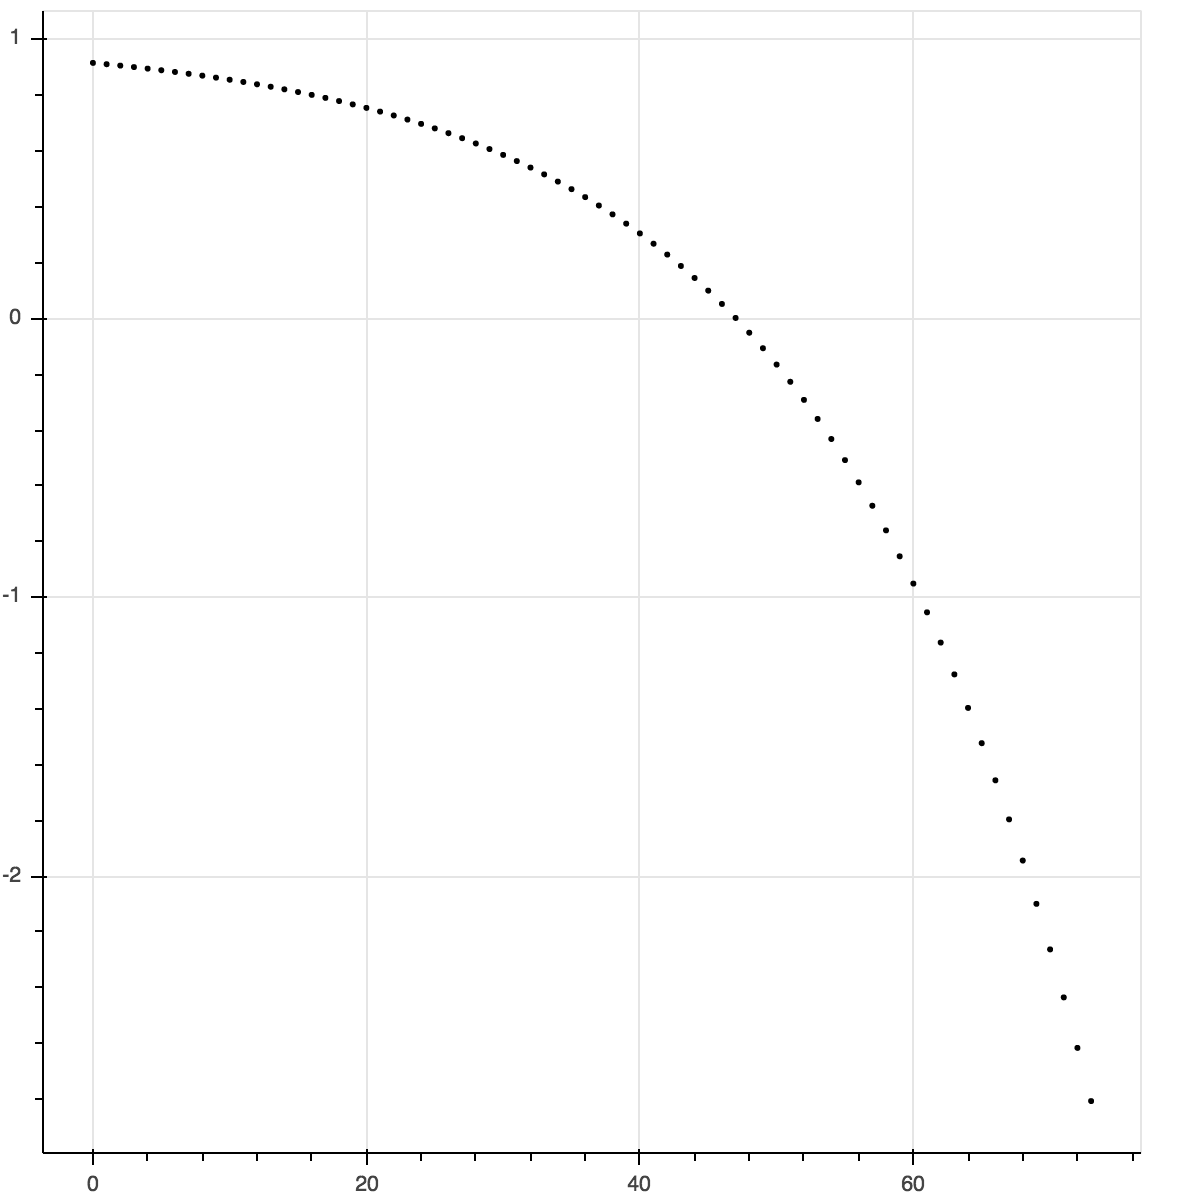
\includegraphics[width=1.0\textwidth]{CartpoleDiscountedNormalizedRewards}}

Therefore, when we multiply \lstinline{discountedRewards} with \lstinline{negLogProb}, the positive head will force the corresponding head entries in \lstinline{negLogProb} to become small, i.e. forcing the head of \lstinline{fc3} to become more like the head of \lstinline{actions}, while the negative tail will force the corresponding tail entries in \lstinline{negLogProb} to become large, i.e. forcing the tail of \lstinline{fc3} to become \emph{less} like the tail of \lstinline{actions}.

\subsection{Why train the network to be unlike the ``Ground Truth''?}

This latter behavior might at first sound like a bad idea: why would you want your network to behave differently than the ``ground truth'' actions?---until we remember that

\large
\begin{quote}
\emph{the tail ``ground truth'' actions aren't that good to begin with: the tail end is when the cart fails to balance the pole and makes it fall over.}
\end{quote}
\normalsize
Making the network behave differently than the ``ground truth'' is akin to trying new things. Sometimes the new behavior will cause a shorter episode, and sometimes a longer one. When it is longer, the tail end of \lstinline{discountedRewards} will be deeper and more negative, thus causing the loss to decrease and the network to favor it.

To emphasize the point, this positive head and negative tail behavior is the reason why we normalize \lstinline{EpisodeRewards} against the \lstinline{mean} and \lstinline{std} in

\footnotesize
\begin{lstlisting}
@staticmethod
def discountNormalizeRewards(EpisodeRewards):
  discountedRewards = np.zeros_like(EpisodeRewards)
  cumulative = 0.0
  for i in reversed(range(len(EpisodeRewards))):
    cumulative = cumulative * GAMMA + EpisodeRewards[i]
    discountedRewards[i] = cumulative

  mean = np.mean(discountedRewards)
  std = np.std(discountedRewards)
  discountedRewards = (discountedRewards - mean) / std

  return discountedRewards
\end{lstlisting}
\normalsize
so that we could have the positive head and negative tail. If we didn't, then \lstinline{discountedRewards} would simply be a list of positive numbers, and when we multiply it with \lstinline{negLogProb} in the \lstinline{loss}, it would cause all entries of \lstinline{negLogProb} to become small, causing \lstinline{fc3} to become more like \lstinline{actions} everywhere, including near the end of the episode when it should behave otherwise and be less like \lstinline{actions}.

\subsection{Summary}

Finally, the loss function

\scriptsize
\begin{lstlisting}
negLogProb = tf.nn.softmax_cross_entropy_with_logits_v2(fc3, actions)
loss = tf.reduce_mean(negLogProb * discountedRewards)
\end{lstlisting}
\normalsize
or in shorthand:
\begin{align*}
L &= - \frac{1}{n} \sum_{i} \< A, \log s(\pi) \> \cdot G \\
G &= \frac{[G_0 \ \cdots \ G_n] - \m}{\s}
\end{align*}
is good for games where the goal is to keep playing, where every step provides a reward.

\begin{question}
Can we use it for other kinds of games?
\end{question}

\end{document}
